% This is file JFM2esam.tex
% first release v1.0, 20th October 1996
%       release v1.01, 29th October 1996
%       release v1.1, 25th June 1997
%       release v2.0, 27th July 2004
%       release v3.0, 16th July 2014
%       release v4.0, 15th June 2017
%   (based on JFMsampl.tex v1.3 for LaTeX2.09)
% Copyright (C) 1996, 1997, 2014, 2017 Cambridge University Press

\documentclass[12pt, a4paper]{article}
\usepackage{graphicx}
% \usepackage{epstopdf, epsfig}

\usepackage{graphicx}
\usepackage{times}
\usepackage{tabularx}
\usepackage{fancyhdr}
\usepackage{pbox}
%\usepackage[utf8]{inputenc}
\usepackage[T1]{fontenc}
\usepackage{amsmath}
\usepackage{setspace}
\usepackage[a4paper, left=25mm, right=25mm, top=30mm, bottom=30mm]{geometry}
\usepackage{titlesec}

% \usepackage[square, comma, sort&compress, numbers]{natbib}
% \bibliographystyle{IEEEtran}
% \usepackage{cite}
\usepackage[style=ieee]{biblatex}



\newcommand{\wideunderline}[2][2em]{%
  \underline{\parbox[t]{#1}{\centering{#2}}}%
}

% \renewcommand\footnotesize{\small}
% \newcommand\indexsize{\@setfontsize\indexsize\@viiipt\@ixpt}
% \renewcommand\scriptsize{\@setfontsize\scriptsize\@viipt\@viiipt}
% \renewcommand\tiny{\@setfontsize\tiny\@vpt\@vipt}
% \renewcommand\large{\@setfontsize\large\@xipt{13}}
% \renewcommand\Large{\@setfontsize\Large\@xivpt{18}}
% \renewcommand\LARGE{\@setfontsize\LARGE\@xviipt{19}}
% \renewcommand\huge{\@setfontsize\huge\@xxpt{25}}
% \renewcommand\Huge{\@setfontsize\Huge\@xxvpt{30}}

\newcommand\SectionSize{\@setfontsize\SectionSize{15}{22.5}}
\newcommand\ArticleSize{\@setfontsize\ArticleSize{14}{21}}
\newcommand\ItemSize{\@setfontsize\ItemSize{12}{18}}

\titleformat{\section}
  {\normalfont\fontsize{15}{22.5}\bfseries}{\thesection}{1em}{}
\titleformat{\subsection}
  {\normalfont\fontsize{14}{21}\bfseries}{\thesubsection}{1em}{}
\titleformat{\subsubsection}
  {\normalfont\fontsize{12}{18}\bfseries}{\thesubsubsection}{1em}{}

% \def\@maketitle{%
%   \newpage
%   \null
%   \vskip 2em%
%   \begin{center}%
%     \LARGE \@title \par
%   \end{center}%
%   \par
%   \vskip 1.5em}


% \redef\@maketitle#1{%
%  \newpage
%  \vspace*{10\p@}%
%  {\centering \sloppy
%   {\normalfont\LARGE\fontswitch\bfseries
%   \put@rapidsHead%
%   \@title@alignment%
%   \@title \par}%
%   \vskip 8\p@ \@plus 2\p@ \@minus 1\p@
%   {\normalfont\large\fontswitch\bfseries\baselineskip=12\p@
%      \@author@alignment%
%      \lowercase{\@author}\par}%
%   \vskip 4\p@ \@plus 1\p@
%   {\normalfont\small
%   \@aff@alignment%
%   \@affiliation \par}%
%   \vskip 8\p@ \@plus 2\p@ \@minus 1\p@
%   %{\normalfont\small (Received \@date)}% x@rem
%   \normalfont\small
%   \@history@alignment%
%   % (Received xx; revised xx; accepted xx)\hfill% x@add
%   \put@absrule
%  \par}%
%  \vskip 8\p@ \@plus 2\p@ \@minus 1\p@
% }

% \renewenvironment{abstract}
%   {\par\normalfont\normalsize\noindent\ignorespaces}
%   {\par\vskip 9\p@ \@plus 1\p@ \@minus 1\p@
% %   \vbox{\centerline{\rule[4\p@]{30pc}{.4\p@}}}
% }


\usepackage{comment}
\usepackage{enumitem}
\usepackage{xcolor}
\definecolor{pink}{RGB}{255, 20, 147}
\usepackage[colorlinks=true,linkcolor=blue,citecolor=green,urlcolor=pink]{hyperref}
\bibliography{reference/reference}

\newtheorem{lemma}{Lemma}
\newtheorem{corollary}{Corollary}
\newcommand{\figref}[1]{[fig:\ref{#1}]}

\title{\fontsize{14pt}{6pt}\selectfont\textbf{Exploring Multi-modal Human Motion Perception for Human-Computer Interaction Systems}} % Set the article title format
\date{} % Set the date to empty to remove it from the title
\author{}

\begin{document}
\newcommand{\GroupProjectTitle}{Research and Implementation of Multimodal Human-Computer Interaction Perception Technology}
\newcommand{\IndividualProjectTitle}{Signal Processing and Modeling of Multimodal Human-Computer Interaction Perception Technology}

\newcommand{\StudentName}{Yijie XU}
\newcommand{\StudentID}{50004147}
\newcommand{\Email}{yxu409@connect.hkust-gz.edu.cn}
\newcommand{\PrimeSupervisor}{Prof. Hui XIONG}
\newcommand{\CoSupervisor}{Prof. Xiaojuan MA}
\newcommand{\HubThrustPrime}{AI Thrust / Information Hub}
\newcommand{\HubThrustCo}{Department of CSE / School of Engineering}
\newcommand{\ProjectMentor}{Dr. Li CHEN}

\begin{titlepage}
    \begin{center}
        \vspace*{1cm}

        \huge

        \textbf{Master Thesis Proposal for MPhil Degree}

        \vspace{3cm}
        
        \begin{minipage}{0.8\textwidth}
            \Large
            \centering

            \begin{tabular}{l@{}ll}
                \textbf{Student Name}\vspace{0.5cm} &     & \wideunderline[18em]{\StudentName} \\
                \textbf{ID Number}\vspace{0.5cm} &     & \wideunderline[18em]{\StudentID} \\
                \textbf{Email}\vspace{1.5cm} &     & \wideunderline[18em]{\Email} \\
                \textbf{Group Project}\vspace{0.5cm} &     & \wideunderline[18em]{{\GroupProjectTitle}} \\ 
                \textbf{Project Mentor}\vspace{1.5cm} &     & \wideunderline[18em]{\ProjectMentor} \\
                \textbf{Individual Project}\vspace{0.5cm}&     & \wideunderline[18em]{{\IndividualProjectTitle}}  \\
                \textbf{Prime Supervisor}\vspace{0.2cm} &     & \wideunderline[18em]{{\PrimeSupervisor}}  \\
                \textbf{Hub/Thrust}\vspace{0.5cm} &     & \wideunderline[18em]{\HubThrustPrime} \\
                \textbf{Co-supervisor}\vspace{0.2cm} &     & \wideunderline[18em]{\CoSupervisor} \\
                \textbf{Hub/Thrust} &     & \wideunderline[18em]{\HubThrustCo} \\
            \end{tabular}

        \end{minipage}

        
        
        \vfill
        
        \LARGE
        \textbf{Division of the RBM} 
             
    \end{center}
 \end{titlepage}

\spacing{1.5}

\maketitle
\begin{abstract}
    Human body motion perception is a crucial research area with significant potential applications, including rehabilitation, human-computer interaction, and sports training. Traditional approaches relying on single modalities, such as video, accelerometer, and gyroscopes, have inherent limitations that can result in inaccuracies and inconsistencies in data collection. To overcome these challenges, we propose using multimodal-based models, specifically Wi-Fi, surface electromyography (sEMG), and video data, which provide complementary information on body posture and movement. Our study explores Wi-Fi signals for indoor positioning and larger-scale movement and sEMG sensors for precise muscle activity, including subtle movements, despite their lack of precise location data due to being directly attached to the skin. My research will focus on the latter two modalities, combined with data collection and model design, to produce outstanding results and contribute to the field.
\end{abstract}
\newpage
\tableofcontents
\newpage
\section{Source of Research Topic, Research Purpose and Significance}

\subsection{The Source of the Topic}
Motion perception is a rapidly growing field of research with numerous potential applications in areas such as rehabilitation, human-computer interaction, and sports training. The ability to accurately perceive and interpret human body posture and movement is essential for developing advanced technologies to improve our daily lives.

Traditional approaches to motion perception have relied on single modalities such as video, accelerometer, and gyroscopes. While these methods have proven effective in certain situations, they also have inherent limitations that can result in inaccuracies and inconsistencies in data collection. For example, video-based methods can be affected by lighting conditions and occlusions, while the accelerometer and gyroscope-based methods may not provide sufficient information about subtle movements.

To overcome these challenges, researchers have begun to explore the use of multimodal-based models that combine multiple sources of information to provide a more comprehensive understanding of human body posture and movement. One promising approach is using Wi-Fi signals for indoor positioning and larger-scale movement detection. Wi-Fi signals can penetrate walls and other obstacles, making them well-suited for indoor environments where traditional methods may struggle.

Another promising modality is surface electromyography (sEMG), which measures the electrical activity muscles produce during contraction. sEMG sensors can provide detailed information about muscle activity, including subtle movements that may be difficult to detect using other methods. However, sEMG sensors lack precise location data due to being directly attached to the skin.

This study proposes combining Wi-Fi, sEMG, and video data to create a multimodal-based model for human motion perception. Our approach leverages the strengths of each modality to provide complementary information about body posture and movement. We will focus on using sEMG and Wi-Fi signals, combined with advanced data collection and model design techniques, on producing outstanding results that contribute to the field.
\subsection{Research Background and Significance}
Human motions are important. It has played a critical role in human communication and social interactions throughout history. Before the invention of writing and language, motions were the primary means of conveying ideas, emotions, and intentions. Even today, motions continue to play an essential role in human communication, adding nuance and meaning to spoken language. Additionally, motion perception is crucial in non-verbal communication, such as interpreting body language and facial expressions. Moreover, the ability to recognize and interpret motions is essential in fields such as psychology, anthropology, and communication studies. Overall, human motion perception is vital to understanding and navigating human interactions and has been integral to human communication throughout history.

After introducing the research background and significance of human motions and motion perceptions, it is important to delve into the development path of motion recognition and the history of using different modalities of sensors and data in human motion perception.

In the domain of human motion recognition, the development path has experienced significant advancements over the years, spanning a range of techniques and methodologies. The early attempts at motion recognition can be traced back to the late 20th century, when researchers initially focused on the analysis of basic motions, such as walking and running, using optical \textbf{Mo}tion \textbf{Cap}ture systems (Mocap). These systems relied on the precise tracking of markers placed on the subject's body, enabling the reconstruction of human motion in three-dimensional space. Although effective, these systems were constrained by their high cost, intrusiveness, and limitations to controlled environments.

With the advent of computer vision and machine learning techniques in the early 21st century, researchers began exploring alternative approaches for motion recognition, which included the use of 2D videos and depth sensors. These methods facilitated the extraction of motion features from image sequences, allowing for the recognition of human motions in more natural and uncontrolled environments. The introduction of the Microsoft Kinect in 2010 further propelled the field, as it provided an affordable, non-intrusive, and easy-to-use depth sensor, which enabled the extraction of accurate skeleton information for human motion analysis.

In parallel with these developments, researchers also began investigating the potential of multimodal approaches, incorporating various sensor modalities and data types for enhanced motion recognition. The integration of \textbf{I}nertial \textbf{M}easurement \textbf{U}nits (IMUs), for instance, allowed for the capture of motion data with high temporal resolution, compensating for the shortcomings of vision-based methods in dynamic and occluded scenarios. Furthermore, the fusion of data from multiple sensors, such as RGB cameras, depth sensors, and IMUs, has demonstrated the potential to improve motion recognition performance, particularly in challenging environments and situations.

One of the most important modalities is inertial sensing, which involves using sensors such as accelerometers and gyroscopes to measure the motion of the body. Inertial sensors are particularly useful for tracking the motion of limbs and joints, and have been used in a variety of applications, from sports training to medical rehabilitation.

Another important modality is \textbf{e}lectro\textbf{m}yo\textbf{g}raphy (EMG), which involves measuring the electrical activity of muscles. EMG has been used to develop systems that can detect subtle muscle movements, such as those involved in sign language or facial expressions.

In recent years, there has also been a growing interest in using wearable devices such as smartwatches and fitness trackers to track human motion. These devices typically incorporate a variety of sensors, including accelerometers, gyroscopes, and heart rate monitors, and can provide a wealth of data about the user's activity levels, sleep patterns, and overall health.

The emergence of deep learning techniques, especially convolutional neural networks (CNNs) and recurrent neural networks (RNNs), has also significantly impacted the field of human motion recognition. These methods have facilitated the automatic learning of hierarchical features from raw sensor data, eliminating the need for manual feature engineering. Researchers have successfully applied these techniques to various modalities, including RGB videos, depth maps, IMU and EMG data, achieving state-of-the-art performance in multiple motion recognition tasks.

In summary, the development path of motion recognition has witnessed considerable advancements over the years, progressing from marker-based optical systems to sophisticated deep learning techniques. The incorporation of multimodal sensor data and fusion techniques has further enhanced the field, allowing for improved motion recognition performance in a wide range of scenarios. As researchers continue to explore new modalities, techniques, and applications, human motion recognition remains a vibrant and evolving area of study, with significant potential for future breakthroughs.

\subsection{Drawbacks}
However, the modalities above have inherent limitations that can result in inaccuracies and inconsistencies in data collection, leading to potential issues in motion recognition. This chapter will cover problems that can occur when using single-modality sensors:
\begin{enumerate}
	\item \textbf{Limited sensing range}: Most single-modality sensors have limited sensing range, which means they can only capture a limited area of the body or environment. For example, a camera-based system can only capture visible motions, while an accelerometer-based system can only capture movements that involve acceleration.
	\item \textbf{Limited accuracy}: Single-modality sensors can also have limited accuracy, especially when it comes to capturing small or subtle movements. For example, accelerometer-based systems may struggle to distinguish between slight variations in movement or sudden stops, leading to inaccuracies in the captured data.
	\item \textbf{Environmental interference}: Single-modality sensors can also be affected by environmental interference, such as lighting conditions, noise, and other sources of interference. For example, a camera-based system may struggle to recognize motions in low-light conditions, while an accelerometer-based system may be affected by vibrations from external sources.
	\item \textbf{Limited depth of analysis}: Single-modality sensors typically capture only one aspect of the motion, such as motion or muscle activity. As a result, the study may be limited regarding the depth and scope of the captured data.
\end{enumerate}

To overcome these challenges, we proposed using multimodal-based models, which combine data from multiple sources to provide a more comprehensive understanding of Human motion recognition. Various sensors, such as Wi-Fi, surface electromyography (sEMG), and video data, can capture complementary information on body posture and movement, leading to more accurate and precise motion recognition results.\\

\section{Literature Review and Analysis}
To introduce our method of combining multi-modal data for motion perception, it is vital to have a research review of using tensors of single modality for motion perception. In this section, we will first cover Wi-Fi, sEMG and vision signals, then have a review of using multi-modal signals.

\subsection{Wi-Fi Sensing for Motion Perceptions}
Wi-Fi sensing for motion perception has gained significant attention in recent years due to the widespread deployment of Wi-Fi networks and the increasing demand for \textbf{H}uman-\textbf{C}omputer \textbf{I}nteraction (HCI) technologies. This section presents a comprehensive review of the state-of-the-art in Wi-Fi sensing for motion perception, including key techniques, methodologies, and applications.

Early works on Wi-Fi sensing for gesture recognition primarily focused on the analysis of \textbf{R}eceived \textbf{S}ignal \textbf{S}trength (RSS) variations caused by human movements. Adib et al. \cite{adib20143d} proposed WiTrack, a through-wall 3D motion tracking system that leverages radio frequency signals to track the motion of a person. Similarly, another work of Adib et al. \cite{adib2013see} utilized Wi-Fi signal reflections to accurately track the position of a person indoors. These systems demonstrated the potential of Wi-Fi signals for motion perception but were limited by the coarse spatial resolution of RSS.

To overcome the limitations of RSS-based systems, researchers began exploring the use of \textbf{C}hannel \textbf{S}tate \textbf{I}nformation (CSI) as a more fine-grained indicator of human motion. Pu et al. \cite{pu2013whole} developed WiSee, a system that exploits CSI to recognize a set of predefined gestures. WiSee demonstrated the feasibility of using Wi-Fi signals for gesture recognition, and numerous researchers have since built upon this work. For example, Wei et al. \cite{abdelnasser2015wigest} proposed WiGest, which leverages CSI phase information to detect the presence of a human and recognize basic gestures. Wu et al. \cite{wang2017phasebeat} introduced PhaseBeat, a CSI-based system that detects micro-movements, such as heartbeat and respiration, through phase information analysis.

\begin{figure}[ht!]
    \centering
    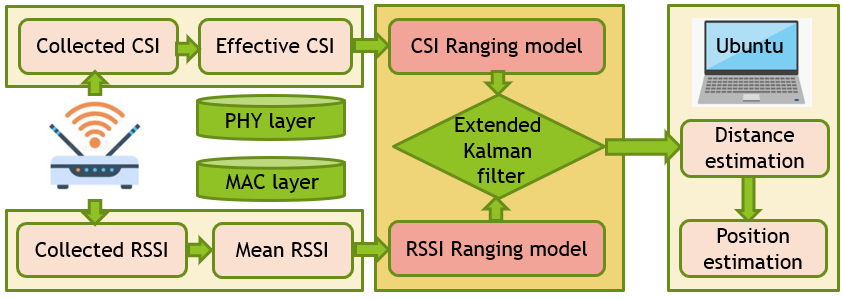
\includegraphics[width=0.6\textwidth]{image/wifi_csi_rsi.png}
    \caption{Wi-Fi sensing by CSI and RSI}
    \label{fig:wifi_csi_rsi}
\end{figure}

Deep learning techniques have also been employed to improve the performance of Wi-Fi sensing systems for gesture recognition. Wang et al. \cite{wang2017cifi} proposed CiFi, which combines \textbf{C}onvolutional \textbf{N}eural \textbf{N}etworks (CNN) and CSI to achieve high recognition accuracy across multiple environments and devices. Li et al. \cite{li2016wifinger} presented WiFinger, a system that leverages deep learning to recognize finger gestures based on CSI data, opening the door to a wide range of HCI applications.

In addition to gesture recognition, Wi-Fi sensing has been explored for various other motion perception applications, such as fall detection, human counting, and localization. Wang et al. \cite{wang2016wifall} designed WiFall, a system that detects falls based on CSI amplitude variations caused by human motion. Wang et al. \cite{wang2014wihear} developed WiHear, which enables Wi-Fi signals to “hear” our talks without deploying any devices.

In summary, Wi-Fi sensing for motion perception has evolved significantly over the past decade, with advancements in both hardware and software techniques. From early works using RSS to more recent studies employing CSI and deep learning, Wi-Fi sensing has shown great potential for a wide range of applications, including gesture recognition, fall detection, and localization. Future research should continue to focus on improving the accuracy, robustness, and generalizability of Wi-Fi sensing systems, as well as exploring novel applications for this promising technology.

\subsection{sEMG Signals for Motion Perception}
Over the past decade, the investigation of \textbf{s}urface \textbf{e}lectro\textbf{m}yo\textbf{g}raphy (sEMG) signals has played a pivotal role in the advancement of motion perception research \cite{Kyeong2022}. Surface electromyography (sEMG) has been widely utilized for various applications, including rehabilitation engineering, human-machine interfaces (HMIs), and motion perception \cite{phinyomark2012feature, ortiz2014osseointegrated}. The development of sEMG-based systems for gesture recognition and motion perception can be traced back to the early 1980s, when researchers began to investigate the potential of sEMG for controlling prosthetic devices \cite{parker2006myoelectric}. As the field progressed, advanced signal processing techniques and machine learning algorithms were introduced to improve the performance of sEMG-based systems.

During the 1990s, researchers focused on improving the accuracy and robustness of sEMG-based gesture recognition. Time-domain features, such as mean absolute value, waveform length, and zero-crossing rate, were commonly used for extracting relevant information from sEMG signals \cite{zecca2002control}. The use of \textbf{A}rtificial \textbf{N}eural \textbf{N}etworks (ANNs) for the classification of sEMG signals started to gain popularity, leading to significant improvements in the recognition of hand gestures and movements \cite{hargrove2008training}.

The rise of support vector machines (SVM) in the 2000s further improved the performance of sEMG-based gesture recognition systems. Alongside the increasing computational power, the combination of SVM classifiers and various feature extraction methods, such as wavelet analysis, allowed for the identification of multiple degrees of freedom in hand and arm movements with high accuracy \cite{englehart1999classification}. The introduction of wearable technology and miniaturization of sEMG sensors further facilitated the development of portable and user-friendly HMIs \cite{castellini2009surface}.

In the 2010s, deep learning techniques, particularly \textbf{C}onvolutional \textbf{N}eural \textbf{N}etworks (CNNs) and \textbf{R}ecurrent \textbf{N}eural \textbf{N}etworks (RNNs), were introduced to sEMG-based gesture recognition and motion perception research. CNNs demonstrated exceptional performance in the classification of sEMG signals, surpassing traditional feature extraction and classification methods \cite{diener2015direct}. RNNs, specifically \textbf{L}ong \textbf{S}hort-\textbf{T}erm \textbf{M}emory (LSTM) networks, showed potential for modeling the temporal dynamics of sEMG signals, leading to improved recognition of complex and time-varying gestures \cite{geng2016gesture}.

Throughout the years, researchers have also explored different approaches for improving the usability and adaptability of sEMG-based systems. Techniques such as transfer learning and domain adaptation have been proposed to address issues related to subject-specificity and variations in sensor placements \cite{du2017surface}. Additionally, the integration of sEMG with other modalities, such as inertial measurement units (IMUs) and vision-based systems, has shown promising results in enhancing gesture recognition and motion perception capabilities \cite{radmand2016high}.

In summary, the historical development of using sEMG signals for gesture recognition and motion perception has seen significant advancements over the years. From the early applications in prosthetic control to the recent developments in deep learning and multimodal systems, sEMG-based gesture recognition and motion perception research continue to evolve and expand, offering new opportunities for rehabilitation, human-machine interaction, and beyond.

\subsection{Vision Signals for Motion Perception}
In this section, we review the literature on the use of vision signals for motion perception. Over the years, computer vision techniques have evolved significantly in their ability to extract and process motion information from visual data, leading to improved performance in gesture recognition tasks.

One of the early developments in the field of computer vision was the introduction of optical flow algorithms for estimating motion in image sequences. These algorithms, such as the Lucas-Kanade method \cite{lucas1981iterative} and the Horn-Schunck method \cite{horn1981determining}, enabled the extraction of motion information from RGB images.

The emergence of depth sensors, such as the Microsoft Kinect, provided a breakthrough in the field of gesture recognition and motion perception. The Kinect captured depth information in addition to RGB data, allowing researchers to develop more robust algorithms that relied on three-dimensional information. Shotton et al. \cite{shotton2011real} proposed a body part labeling algorithm using depth information, which laid the groundwork for subsequent research on gesture recognition.

Another significant development was the introduction of \textbf{C}onvolutional \textbf{N}eural \textbf{N}etworks (CNNs) for motion perception. The success of CNNs in image classification tasks \cite{krizhevsky2017imagenet} led researchers to investigate their application for gesture recognition. Ji et al. \cite{ji20123d} introduced 3D CNNs for action recognition, utilizing both spatial and temporal information from video sequences. This approach was further improved by the use of two-stream CNNs, which separately processed RGB and optical flow data before fusing them for action recognition \cite{simonyan2014two}.

Depth-based approaches were also enhanced by the introduction of skeleton-based methods for gesture recognition. These methods utilized the 3D positions of human joints to recognize gestures, which provided a more compact and computationally efficient representation of motion information. Yang and Tian \cite{yang2012eigenjoints} proposed the EigenJoints method, while Wang et al. \cite{wang2012mining} introduced the Actionlet Ensemble Model, both of which achieved state-of-the-art performance in gesture recognition tasks.

With the advancements in deep learning, researchers began to explore the combination of RGB and depth data for motion perception. One such approach is the fusion of multi-modal data at different levels of the network architecture. For example, Song et al. \cite{song2017end} presented an end-to-end trainable deep architecture that fused RGB and depth data in a hierarchical manner for gesture recognition.

More recently, researchers have begun to explore the use of \textbf{R}ecurrent \textbf{N}eural \textbf{N}etworks (RNNs) for motion perception. RNNs, such as \textbf{L}ong \textbf{S}hort-\textbf{T}erm \textbf{M}emory (LSTM) networks \cite{graves2012long} and \textbf{G}ated \textbf{R}ecurrent \textbf{U}nits (GRUs) \cite{cho2014learning}, are well-suited for modeling temporal sequences and have shown promising results in gesture recognition tasks \cite{donahue2015long}.

\begin{figure}[ht!]
    \centering
    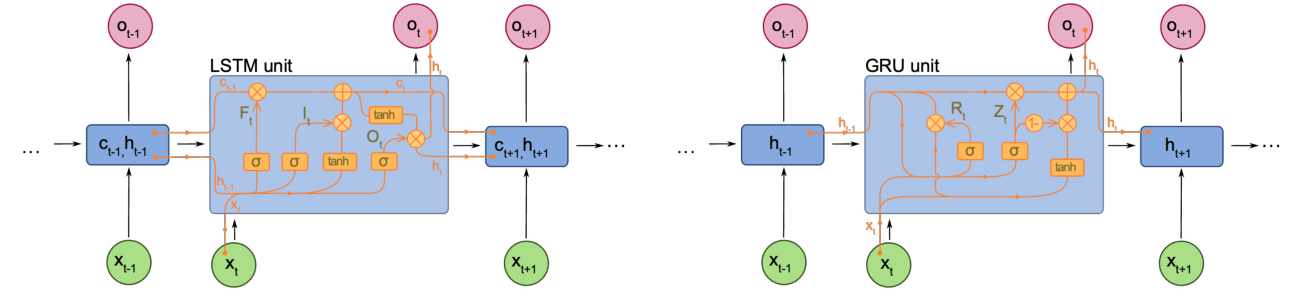
\includegraphics[width=1.0\textwidth]{image/lstm_gru.pdf}
    \caption{Long Short-Term Memory networks and Gated Recurrent Units}
    \label{fig:lstm_gru}
\end{figure}

In conclusion, the history of computer vision techniques for motion perception has seen significant advancements, from early optical flow algorithms to the use of deep learning methods that combine RGB and depth information. These developments have led to increasingly accurate and robust algorithms for motion perception, paving the way for further research in this domain.


\subsection{Analysis of the Literature Review}
The literature review above provides valuable insights into the research advancements and limitations of using Wi-Fi, sEMG, and vision signals for motion perception. In recent years, researchers have extensively investigated the use of Wi-Fi signals for motion perception, providing non-intrusive and ubiquitous sensing technology for indoor monitoring and localization applications. While Wi-Fi signals present certain limitations, including poor environmental adaptability and low resolution, they remain a promising instrument for researchers and developers.

\textbf{S}urface \textbf{e}lectro\textbf{m}yo\textbf{g}raphy (sEMG) signals have also gained significant attention for motion perception research, owing to their advantages of electromechanical delay and muscle activation information. Various studies have utilized sEMG signals to recognize discrete motion intentions, hand gestures, and motion recognition. Deep learning models have been employed to augment the precision of motion recognition, and these advancements hold significant potential for improving prosthesis control, rehabilitation, and human-computer interaction in individuals with disabilities, such as upper-limb amputees.

Computer vision technology has facilitated the recognition of hand gestures and body movements, with techniques from image processing, machine learning, and deep learning employed to recognize and classify gestures. The development of computer vision technology for motion perception holds the potential to revolutionize human interactions with machines and virtual environments. However, researchers face challenges such as variability in hand and body appearance, motion, size, and shape.\\

\newpage
\section{Main Content of Research}
Our principal endeavor is to \textbf{pioneer} the investigation and implementation of multi-modal human-computer interaction perception technology, with a focus on its application in diverse scenarios, such as human motion perception. This objective encompasses two primary components: the exploration of viable research avenues and the determination of suitable implementation strategies. The initial subsection will address the core aspects of employing Wi-Fi, sEMG and vision signals for motion perception, while the subsequent subsection will delineate the advancements in implementation.

\subsection{Research Avenues}
In this subsection, we will explore the main research directions for multi-modal human-computer interaction perception technology, focusing on the integration of Wi-Fi, sEMG, and vision signals for motion perception. The primary goal of this research is to develop a comprehensive framework that combines the strengths of each modality to enhance the overall performance of the system in terms of accuracy, reliability, and efficiency.

\subsubsection{Wi-Fi-based Motion Perception}

Wi-Fi signals have shown great potential in human motion perception due to their ability to penetrate walls and non-metallic objects, thus enabling \textbf{N}on-\textbf{L}ine-\textbf{O}f-\textbf{S}ight (NLOS) monitoring. Research in this area will focus on developing novel algorithms and techniques to accurately estimate human body movements based on Wi-Fi signal variations. This includes investigating machine learning and deep learning approaches for modeling and interpreting Wi-Fi signal characteristics, as well as exploring methods for mitigating the impact of environmental factors on Wi-Fi-based motion perception.

\subsubsection{sEMG-based Motion Perception}

Surface electromyography (sEMG) offers a direct and precise means of capturing muscle activities associated with human movements. Research in this area will concentrate on enhancing the quality of sEMG signals through advanced signal processing techniques, such as filtering, feature extraction, and noise reduction. Additionally, we will investigate machine learning algorithms, including supervised and unsupervised learning, to classify and interpret sEMG signals for various motion perception tasks. This research will also explore the potential of incorporating wearable devices and sensors to improve the overall performance of sEMG-based motion perception systems.

\subsubsection{Vision-based Motion Perception}

Vision-based motion perception techniques rely on visual information from cameras or other optical devices to estimate human movements. Research in this domain will focus on improving the robustness and accuracy of vision-based methods by employing advanced computer vision techniques, such as optical flow, feature matching, and deep learning-based approaches like convolutional neural networks (CNNs) and recurrent neural networks (RNNs). Furthermore, we will explore methods for addressing challenges associated with occlusions, varying lighting conditions, and real-time processing requirements.

\subsubsection{Fusion of Multi-modal Signals for Motion Perception}

The integration of Wi-Fi, sEMG, and vision signals is crucial for developing a comprehensive multi-modal human-computer interaction perception system. Research in this area will focus on designing efficient fusion algorithms that can effectively combine information from different modalities to enhance the overall performance of the system. This includes investigating various fusion strategies, such as data-level, feature-level, and decision-level fusion, as well as exploring the use of machine learning techniques, such as ensemble learning and multi-task learning, to optimize the fusion process. We will try to use the State-of-the-Art transformer architecture in this problem. One existing example is \textbf{UniT}\cite{hu2021unit}, a unified Transformer model to simultaneously learn the most prominent tasks across different domains, ranging from object detection to natural language understanding and multimodal reasoning. Additionally, we will examine methods for selecting and weighting the contributions of each modality based on their reliability and relevance to specific motion perception tasks.

\begin{figure}[ht!]
    \centering
    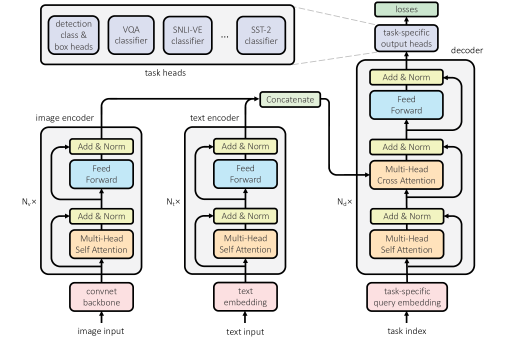
\includegraphics[width=0.5\textwidth]{image/unit.png}
    \caption{An overview of our UniT model, which jointly handles a wide range of tasks in different domains with a unified transformer encoder-decoder architecture.}
    \label{fig:unit}
\end{figure}

\subsubsection{Evaluation and Validation}

A thorough evaluation of the proposed multi-modal human-computer interaction perception system is essential for ensuring its effectiveness and reliability in real-world scenarios. Research in this area will include the development of suitable performance metrics and benchmark datasets for assessing the accuracy, robustness, and efficiency of the integrated system. Moreover, we will conduct rigorous validation studies, including comparative analyses with existing single-modality and multi-modal systems, as well as user studies to evaluate the usability and user satisfaction of the proposed framework.

In summary, this research aims to advance the state-of-the-art in multi-modal human-computer interaction perception technology by focusing on the integration of Wi-Fi, sEMG, and vision signals for motion perception. The proposed research directions will collectively contribute to the development of a comprehensive and reliable framework that can effectively facilitate various human motion perception tasks and applications.
\begin{comment}
	The initial phase in developing a novel generation of human-computer interaction systems involves identifying swifter, more intuitive, and effortless interaction interfaces, which not only permit rapid and accurate comprehension of human intent but also refrain from imposing additional physical or educational burdens upon users. Presently, signals employed for intent recognition can be broadly classified into two categories: non-physiological signals and physiological electrical signals. Non-physiological signals, which encompass imagery, videos, and mechanical inputs (e.g., keyboards and control buttons), have already been extensively integrated into everyday life. However, current non-physiological signal interfaces remain hindered by issues of inconvenient portability and a lack of natural intuitiveness. Physiological electrical signals, in contrast, provide an instinctive and natural representation of user intent and, with their ease of collection, have garnered increasing attention within the realm of human-computer interaction. The primary physiological electrical signals utilized for human-computer interaction include electroencephalograms (EEG), electromyograms (EMG), and electrooculograms (EOG).
	
	Electroencephalograms encapsulate the most extensive range of human intent, yet current acquisition techniques remain incapable of noninvasively collecting high-quality signals. Surface electromyography (sEMG) is frequently regarded as a filter and amplifier for motor intent information within EEG signals, generated by motor neurons in muscles and formed on the skin's surface through the temporal and spatial summation of action potentials, encompassing abundant motor intent information. sEMG enables the collection of high-quality signals from various body parts through noninvasive means, depending on the type of movement information required. As action potentials precede muscle movement, information can be transmitted externally before the actual movement occurs, facilitating the development of lower-latency interaction methods. Consequently, sEMG serves as an exceptional window into motor intent.
	
	At present, two primary methods exist for extracting motor intent based on electromyographic signals. The first involves utilizing classification algorithms to categorize electromyographic signals, generating discrete motion information that can function as switch signals in human-computer interactions. However, as human-computer interaction scenarios grow increasingly complex, this rudimentary classification approach no longer suffices for everyday use. The second method employs regression techniques to extract continuous motion intent information (e.g., joint angles at each moment), providing a more natural and precise solution for intricate human-computer interaction scenarios, albeit presenting greater challenges and demands for decoding algorithm accuracy.
	
	While the advantages of sEMG for human-computer interaction are evident, accurately and swiftly decoding continuous intent information within sEMG remains a formidable challenge. The primary obstacles faced include:
	\begin{enumerate}[(1)]
		\item the need for more refined surface electromyographic feature design for continuous motion estimation compared to discrete motion pattern classification;
		\item current decoding algorithms lacking sufficient accuracy and robustness for practical applications;
		\item the limitation of algorithm complexity due to surface electromyography often being used in outdoor and mobile scenarios, which require mobile hardware platforms.
	\end{enumerate}
	
	With the advent of artificial intelligence, deep learning algorithms have been widely applied in the fields of imagery, video, audio, and text, significantly enhancing societal productivity. The strengths of deep learning algorithms lie in their exceptional feature extraction capabilities and the effective utilization of a multitude of parameters to approximate arbitrary functions. Nonetheless, compared to image classification and speech recognition, the realm of continuous motion estimation using electromyography still lacks real-time performance and accuracy in deep learning networks. The application methodologies and topological structures of deep learning networks in continuous motion estimation warrant further exploration.
	
	In the realm of motion perception, visual signals also play an integral and irreplaceable role, offering a wealth of information to facilitate human-computer interaction. As a continuation of the aforementioned analysis, this study delves into the application of visual signals, specifically examining their utility, challenges, and potential advancements.
	
	Visual signals, encompassing data from sources such as cameras and depth sensors, have been widely adopted in various human-computer interaction scenarios. These signals enable the tracking and interpretation of human motion, allowing for a diverse array of interactive applications, ranging from gesture recognition and virtual reality to robotics and remote control. The main advantages of utilizing visual signals include their noninvasive nature, the ease of data acquisition, and the vast amount of information they can provide.
	
	Despite the substantial benefits, several challenges persist in the application of visual signals for motion perception. The primary obstacles include: 
	\begin{enumerate}[(1)]
		\item the susceptibility of visual data to environmental factors, such as lighting conditions, occlusions, and background noise, which can adversely impact the accuracy and robustness of motion analysis;
		\item the high computational cost and latency associated with processing large volumes of visual data, which can impede real-time performance in certain applications;
		\item the potential issues related to user privacy, as visual data often captures sensitive personal information.
	\end{enumerate}
	
	To address these challenges and further enhance the application of visual signals in motion perception, several research directions are proposed: 
	\begin{enumerate}[(1)]
		\item the development of advanced computer vision and machine learning algorithms to improve the extraction of motion features, taking into account the complexities of human movement and environmental factors;
		\item the exploration of multi-modal fusion techniques, integrating visual signals with other sources of information, such as surface electromyography or inertial sensors, to augment the accuracy and robustness of motion perception;
		\item the optimization of computational models, leveraging hardware acceleration and distributed computing to reduce latency and enhance real-time performance;
		\item the implementation of privacy-preserving mechanisms to protect user data, such as encrypted computation and decentralized storage.
	\end{enumerate}
	
	In conclusion, visual signals hold immense potential in the domain of motion perception, enabling a plethora of human-computer interaction applications. By addressing the existing challenges and pursuing the proposed research directions, it is anticipated that the efficacy and scope of visual signals in motion perception will be significantly bolstered, paving the way for more sophisticated and immersive human-computer interaction experiences.
\end{comment}
\subsection{Implementation Strategies}
In this section, some scheduled implementions will be introduced. We will also discuss some practical scenarios and further working directions.

\subsubsection{Real-Time Multi-Modal Data Collection and Analysis Platform}
In this proposal, we aim to design and implement a real-time multi-modal data collection and analysis platform, which will integrate three distinct modalities: surface electromyography (sEMG), Wi-Fi-based positioning systems, and computer vision. The purpose of this platform is to facilitate the seamless collection, processing, and analysis of multi-modal data for motion perception and classification tasks in various applications, such as rehabilitation, sports performance analysis, and human-computer interaction.

\subsubsection{Multi-Modal Data Collection and Categorization}
To ensure the effectiveness and robustness of our proposed multi-modal model, it is crucial to collect adequate data representing different actions and modalities. The data collection process will involve recruiting participants from diverse backgrounds, performing a wide range of actions, and capturing the corresponding sEMG, Wi-Fi, and vision signals. These data samples will then be stored into different categories, which will be defined based on the type of action, the context of the action, and the modality being analyzed. This systematic categorization will enable the development of more accurate and efficient motion perception and classification algorithms, as well as facilitate the evaluation of the model's performance across different modalities and action types. An example of such dataset \cite{Atzori2014} could be studied and such publication is expected.

\subsubsection{Multi-Modal Model Development for Motion Perception}
Upon the completion of the data collection and categorization phase, we will proceed to develop a multi-modal model for motion perception and classification. The proposed model will leverage state-of-the-art transformer-based architectures, which have demonstrated remarkable success in various machine learning tasks, including natural language processing, computer vision, and time-series analysis. These transformer-based models are particularly well-suited for our application, as they can effectively capture the complex relationships and dependencies among the different modalities.

In order to develop a comprehensive and robust multi-modal model, we will also investigate existing works in the field. Some notable studies to consider include those that focus on fusing sEMG and computer vision signals for gesture recognition \cite{Atzori2014} (which is currently my focus), as well as those that explore Wi-Fi-based human activity recognition \cite{wang2016wifi}. By building upon these existing works and incorporating transformer-based architectures, our proposed model aims to achieve high performance in motion perception and classification across all three modalities.

\subsubsection{Future Directions and Considerations}
As we progress in our research, we will continuously evaluate our multi-modal model's performance and discuss potential improvements and extensions. One possible direction for future work is to explore the integration of additional modalities, such as \textbf{I}nertial \textbf{M}easurement \textbf{U}nits (IMUs) or depth sensors, which is a popular direction to form RGB-D signals, to further enhance the model's accuracy and robustness. Another avenue to consider is the development of adaptive algorithms that can dynamically adjust the model's parameters based on the specific context or application, ensuring optimal performance across various settings.

Moreover, we will investigate the potential of our multi-modal model for real-world applications, such as rehabilitation programs, sports training, and virtual or augmented reality systems. By closely collaborating with domain experts and end-users, we aim to ensure that our research contributes to the development of practical, effective, and user-friendly solutions that address pressing challenges in motion perception and classification.\\

\newpage
\section{Accomplished Work}
This section outlines the work completed since the initiation of this research project in February 2023. The progress thus far includes three distinct chapters, each focusing on one of the three modalities employed in our multi-modal human-computer interaction perception technology.

\subsection{Wi-Fi Signals} I have successfully developed a Wi-Fi signal capturing platform \figref{fig:wifi}, comprising both hardware and software components. This platform enables the efficient collection and processing of Wi-Fi signals, facilitating the investigation of their potential applications in human motion perception tasks.

\begin{figure}[ht!]
    \centering
    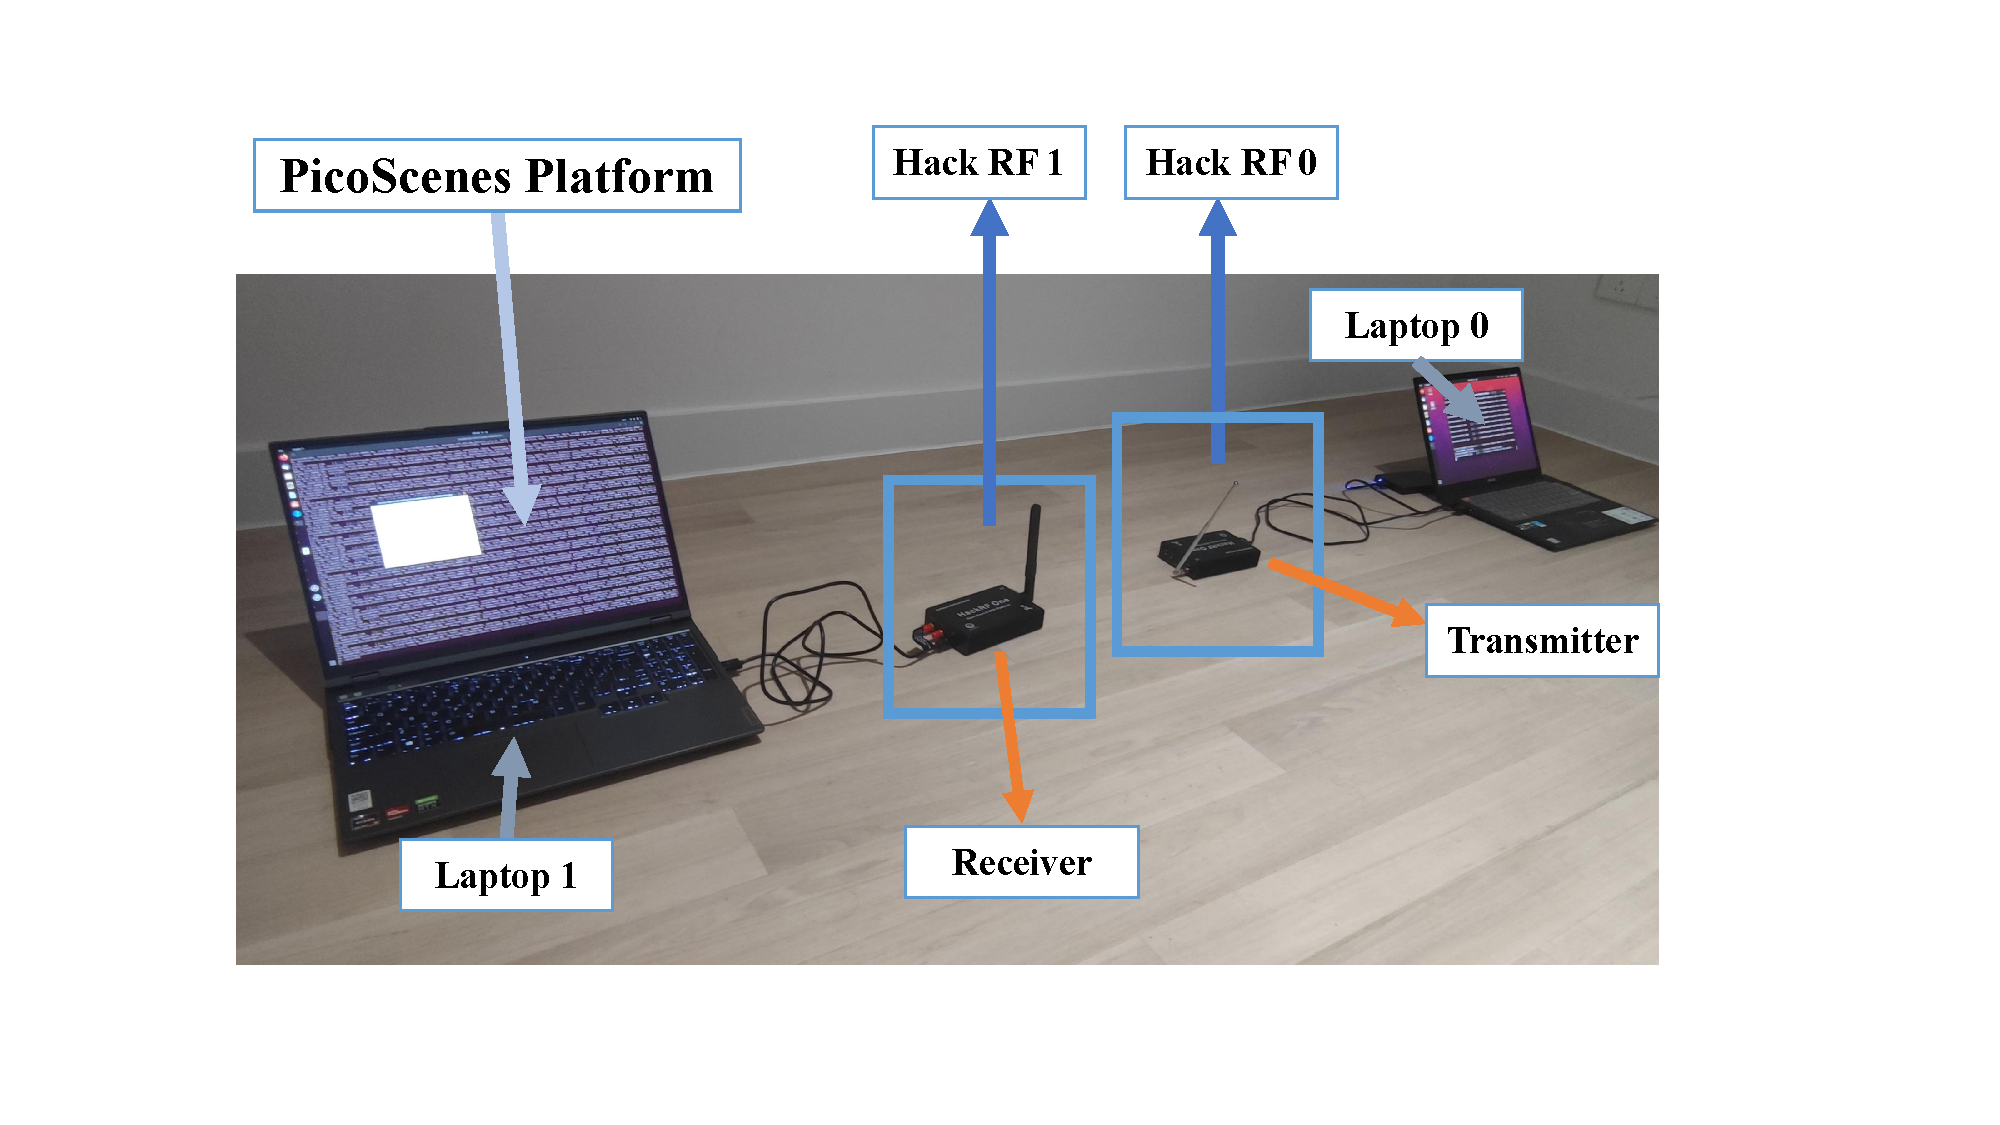
\includegraphics[width=1.0\textwidth]{image/wifi.pdf}
    \caption{Wi-Fi signals capturing system}
    \label{fig:wifi}
\end{figure}


\subsubsection{Hardware Side}
For the hardware component, we have selected the HackRF One hardware, a sophisticated software-defined radio (SDR) peripheral that facilitates the transmission and reception of radio signals within the frequency range of 1 MHz to 6 GHz \cite{ossmann2018hackrf}. The HackRF One boasts numerous advantages, such as an extensive frequency range, high resolution, and compatibility with a diverse array of open-source software. Furthermore, it features an open-source hardware design, which affords the opportunity for potential customization and enhancement in future research endeavors. We have procured two HackRF One units, designating one for transmission and the other for reception. Despite encountering challenges in optimizing the hardware settings for specific frequency bands and mitigating interference, we have accomplished the foundational work necessary for environmental information collection.

In parallel, we have conducted an extensive literature review on Wi-Fi-based human activity recognition techniques \cite{wang2016wifi}, delving into methodologies for augmenting signal quality, such as adaptive filtering and noise reduction algorithms \cite{karedal2007measurement}. The insights gleaned from this review will prove invaluable for refining our Wi-Fi signal collection platform and improving the quality of the data obtained.

\subsubsection{Software Side}
For the software side, we selected the PicoScenes software \figref{fig:picoscenes}, a versatile and high-performance Wi-Fi sensing platform designed for capturing \textbf{C}hannel \textbf{S}tate \textbf{I}nformation (CSI) \cite{jiang2022picoscenes}. We have familiarized ourselves with various APIs and learned how to utilize MATLAB and Python toolboxes for parsing the CSI files captured. Some challenges of using this software include limited documentation, closed-source nature, and compatibility issues. Nevertheless, we will continue exploring more APIs to customize the software for additional use cases.

To further improve the software side, we have investigated various techniques for Wi-Fi signal processing and feature extraction, such as \textbf{P}rincipal \textbf{C}omponent \textbf{A}nalysis (PCA) and \textbf{D}iscrete \textbf{W}avelet \textbf{T}ransform (DWT) \cite{palipana2018falldefi}. This will enable us to extract meaningful information from the collected Wi-Fi signals and facilitate their integration with other modalities in the multi-modal model.

\begin{figure}[ht!]
    \centering
    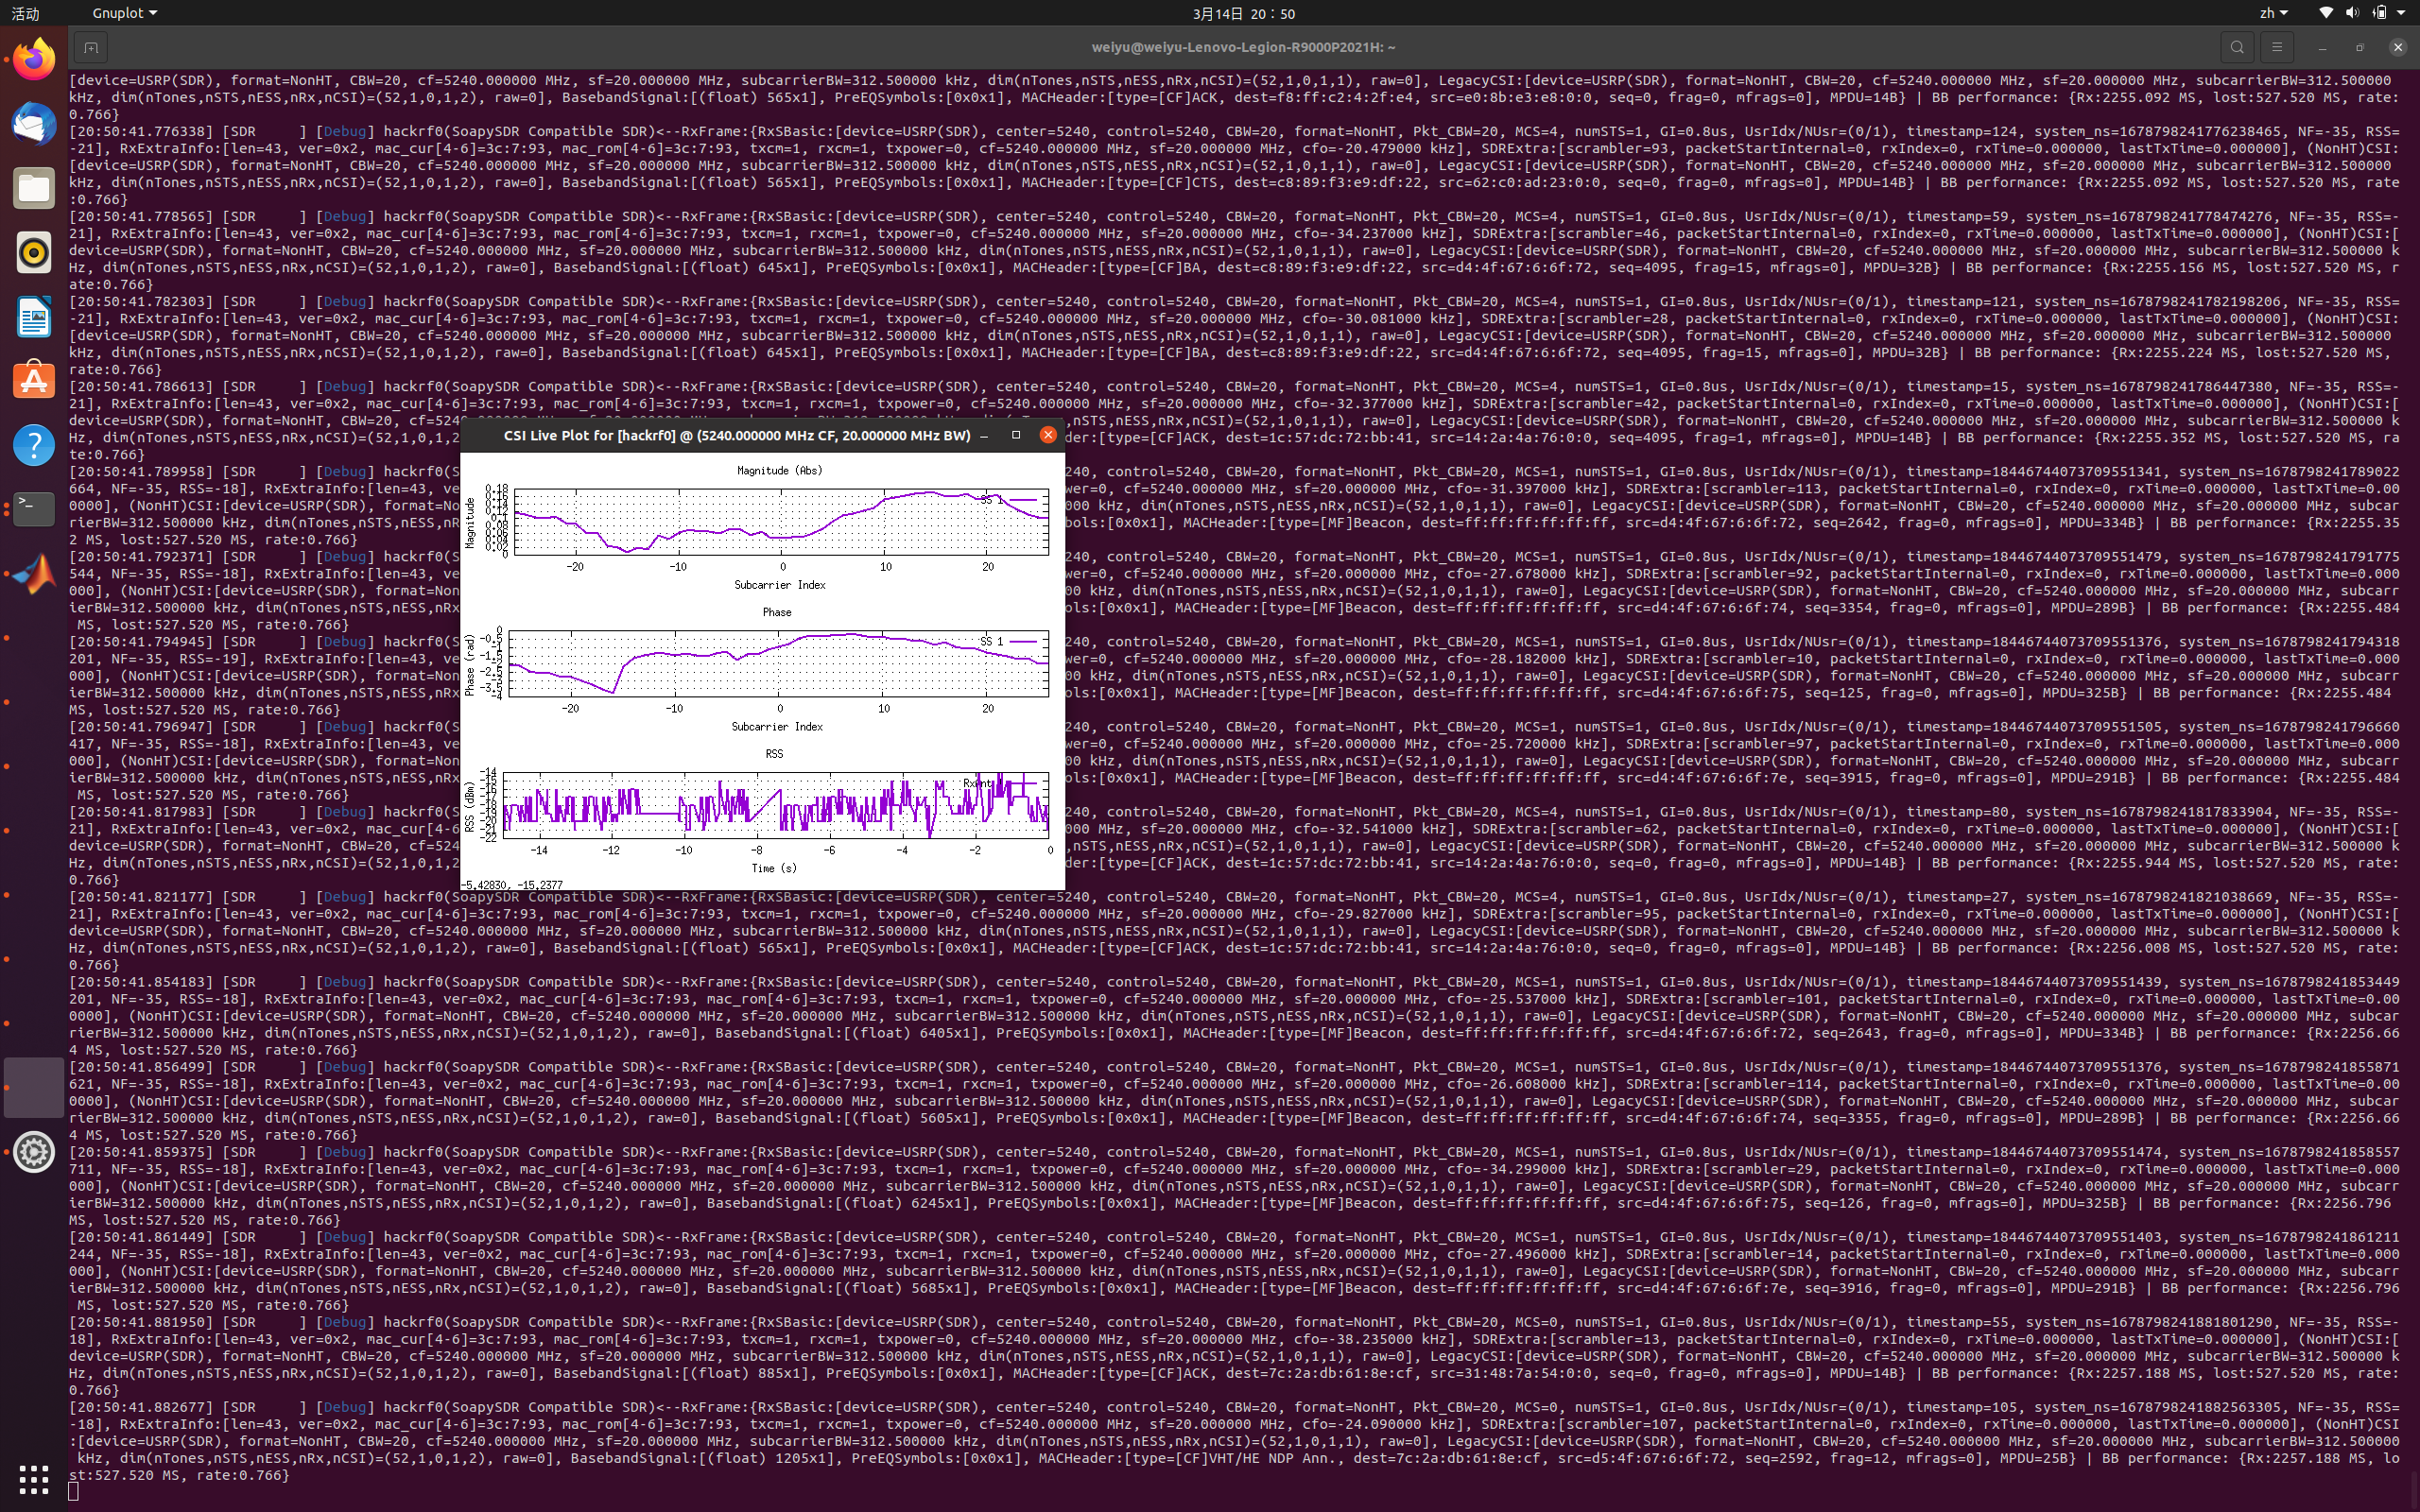
\includegraphics[width=0.75\textwidth]{image/PicoScenes.png}
    \caption{Real-time CPI capturing by PicoScenes}
    \label{fig:picoscenes}
\end{figure}

\subsection{Vision Signals}
We have successfully implemented the FFmpeg API to capture videos with different parameters, such as video codec, width, height, resolution, and bitrate. The advantages of FFmpeg include its open-source nature, cross-platform compatibility, and extensive functionality for processing video and audio files \cite{tomar2006converting}. The flexibility and efficiency of FFmpeg make it an ideal choice for capturing vision signals in various settings, as it allows for real-time video processing and easy integration with other tools and libraries.

Additionally, we have utilized the Google MediaPipe library to recognize human hands. MediaPipe offers several advantages compared to other projects, such as open-source access, high performance, and a modular framework for building multimodal machine learning applications \cite{lugaresi2019mediapipe}. By leveraging the capabilities of MediaPipe, we can efficiently detect and track hand gestures and poses, which will be crucial for our multi-modal model's motion perception and classification tasks.

Furthermore, we have reviewed recent advancements in computer vision techniques for human activity recognition, such as \textbf{C}onvolutional \textbf{N}eural \textbf{N}etworks (CNNs) and \textbf{R}ecurrent \textbf{N}eural \textbf{N}etworks (RNNs) \cite{tran2015deep}. These insights will help inform the development of our vision-based motion perception and classification algorithms and ensure that our multi-modal model leverages state-of-the-art techniques.

\subsection{sEMG signals}
We have rewritten the API provided by \href{https://www.biometricsltd.com/}{Biometrics Ltd}, thereby enhancing performance and enabling access to more information from the underlying hardware. Moreover, we are currently reviewing research articles on using sEMG signals for gesture recognition and motion perception \cite{phinyomark2018usefulness}. This will inform our proposed models, leading to higher performance and accuracy in these tasks.

To ensure the quality of the collected sEMG data, we have investigated various techniques for signal preprocessing, such as filtering, normalization, and segmentation \cite{al-timemy2016classification}. Implementing these techniques will help minimize noise and artifacts in the sEMG signals and facilitate extracting meaningful features for motion perception and classification.

In addition, we have explored feature extraction methods specifically tailored for sEMG signals, such as time-domain, frequency-domain, and time-frequency domain features \cite{tuncer2020surface}. Understanding the advantages and drawbacks of these methods will enable us to select the most appropriate features for our multi-modal model and ensure its effectiveness in capturing the nuances of muscle activation patterns.

Lastly, we have examined machine learning algorithms and deep learning architectures that have been successfully applied to sEMG-based gesture recognition and motion perception tasks, such as \textbf{S}upport \textbf{V}ector \textbf{M}achines (SVMs), \textbf{A}rtificial \textbf{N}eural \textbf{N}etworks (ANNs), and \textbf{C}onvolutional \textbf{N}eural \textbf{N}etworks (CNNs) \cite{zhai2017self}. This knowledge will inform the development of our sEMG-based motion perception and classification algorithms and contribute to the overall performance of the multi-modal model.

\begin{figure}[ht!]
    \centering
    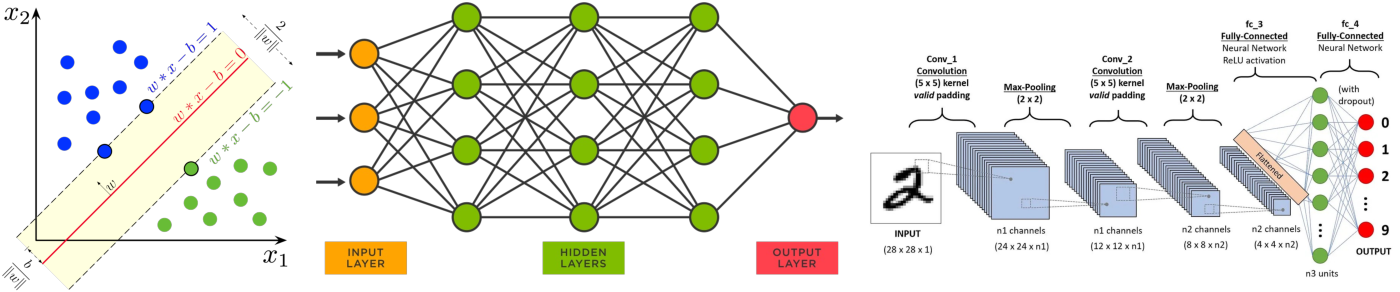
\includegraphics[width=1.0\textwidth]{image/svm_ann_cnn.pdf}
    \caption{Structure of SVM, ANN and CNN}
    \label{fig:svm_ann_cnn}
\end{figure}

We have also completed the first-stage establishment of the online data collection and analysis platform. It currently captures real-time sEMG and vision signals through web interfaces. Integration of Wi-Fi signals is still in progress. As we continue to refine and enhance each platform component, we expect to create a robust and efficient system capable of facilitating high-quality multi-modal data collection and analysis for a wide range of applications.

\newpage
\section{Research Plan, Expected Objectives, and Results}

\subsection{Research Plan}

The research plan for the multi-modal human-computer interaction perception technology project will be carried out in a systematic manner. The plan includes the following steps:

\begin{enumerate}
	\item Literature review and state-of-the-art analysis: Thoroughly review existing literature and research on Wi-Fi, sEMG, and vision-based motion perception, as well as multi-modal fusion techniques.
	\item Development of methodologies and algorithms: Design and implement novel algorithms and techniques for each modality and the fusion process, leveraging the insights gained from the literature review.
	\item Evaluation and validation: Develop performance metrics, benchmark datasets, and conduct comparative analyses with existing methods to assess the effectiveness and reliability of the proposed framework.
	\item User studies and applications: Evaluate the usability and user satisfaction of the integrated system through user studies and explore potential applications in various scenarios.
	\item Dissemination of results: Publish research findings in peer-reviewed journals and conferences, and contribute to open-source software projects related to multi-modal human-computer interaction perception technology.
\end{enumerate}

\subsection{Expected Objectives and Research Achievements}

Upon the completion of this research project, we expect to achieve the following objectives and research accomplishments:

\begin{itemize}
	\item A comprehensive understanding of the state-of-the-art in Wi-Fi, sEMG, and vision-based motion perception techniques, as well as multi-modal fusion strategies.
	\item Development of novel algorithms and techniques for accurate and efficient motion perception using Wi-Fi, sEMG, and vision signals, individually and in combination.
	\item A robust and reliable multi-modal human-computer interaction perception framework that can effectively integrate Wi-Fi, sEMG, and vision signals for various motion perception tasks.
	\item Rigorous validation of the proposed framework, demonstrating its superior performance compared to existing single-modality and multi-modal systems.
	\item Identification of potential applications of the integrated system in various scenarios, such as rehabilitation, sports, and entertainment.
	\item Publication of research findings in high-impact journals and conferences, and contributions to the broader research community through open-source projects.
\end{itemize}

\subsection{Time Scheme}

The following time scheme outlines the timeline for the research project, starting on March 19th, 2023, and concluding by August 2024.

\begin{itemize}
	\item \textbf{March 2023 - June 2023:} Conduct literature review and state-of-the-art analysis.
	\item \textbf{July 2023 - December 2023:} Develop methodologies and algorithms for each modality and the fusion process.
	\item \textbf{January 2024 - April 2024:} Evaluate and validate the proposed framework, including comparative analyses and user studies.
	\item \textbf{May 2024 - June 2024:} Explore potential applications and finalize research findings.
	\item \textbf{July 2024 - August 2024:} Prepare and submit research publications, and contribute to open-source projects.
\end{itemize}

By following this structured research plan and time scheme, we aim to complete the proposed research project within the designated timeframe, leading to significant advancements in multi-modal human-computer interaction perception technology and contributing to the body of knowledge in this domain.

\newpage
\section{Required Conditions and Resources}
Having our budget plan \figref{fig:budget_plan} approved by RBM, we have commenced the procurement process \figref{fig:procurement} and have submitted a comprehensive list of first-stage products and resources required for the successful execution of our project. Prior to submission, these resources underwent thorough scrutiny and evaluation, based on their quality and competitive pricing. Currently, we are awaiting the Division of RBM's approval to proceed to the next phase of procurement.

\begin{figure}[ht!]
    \centering
    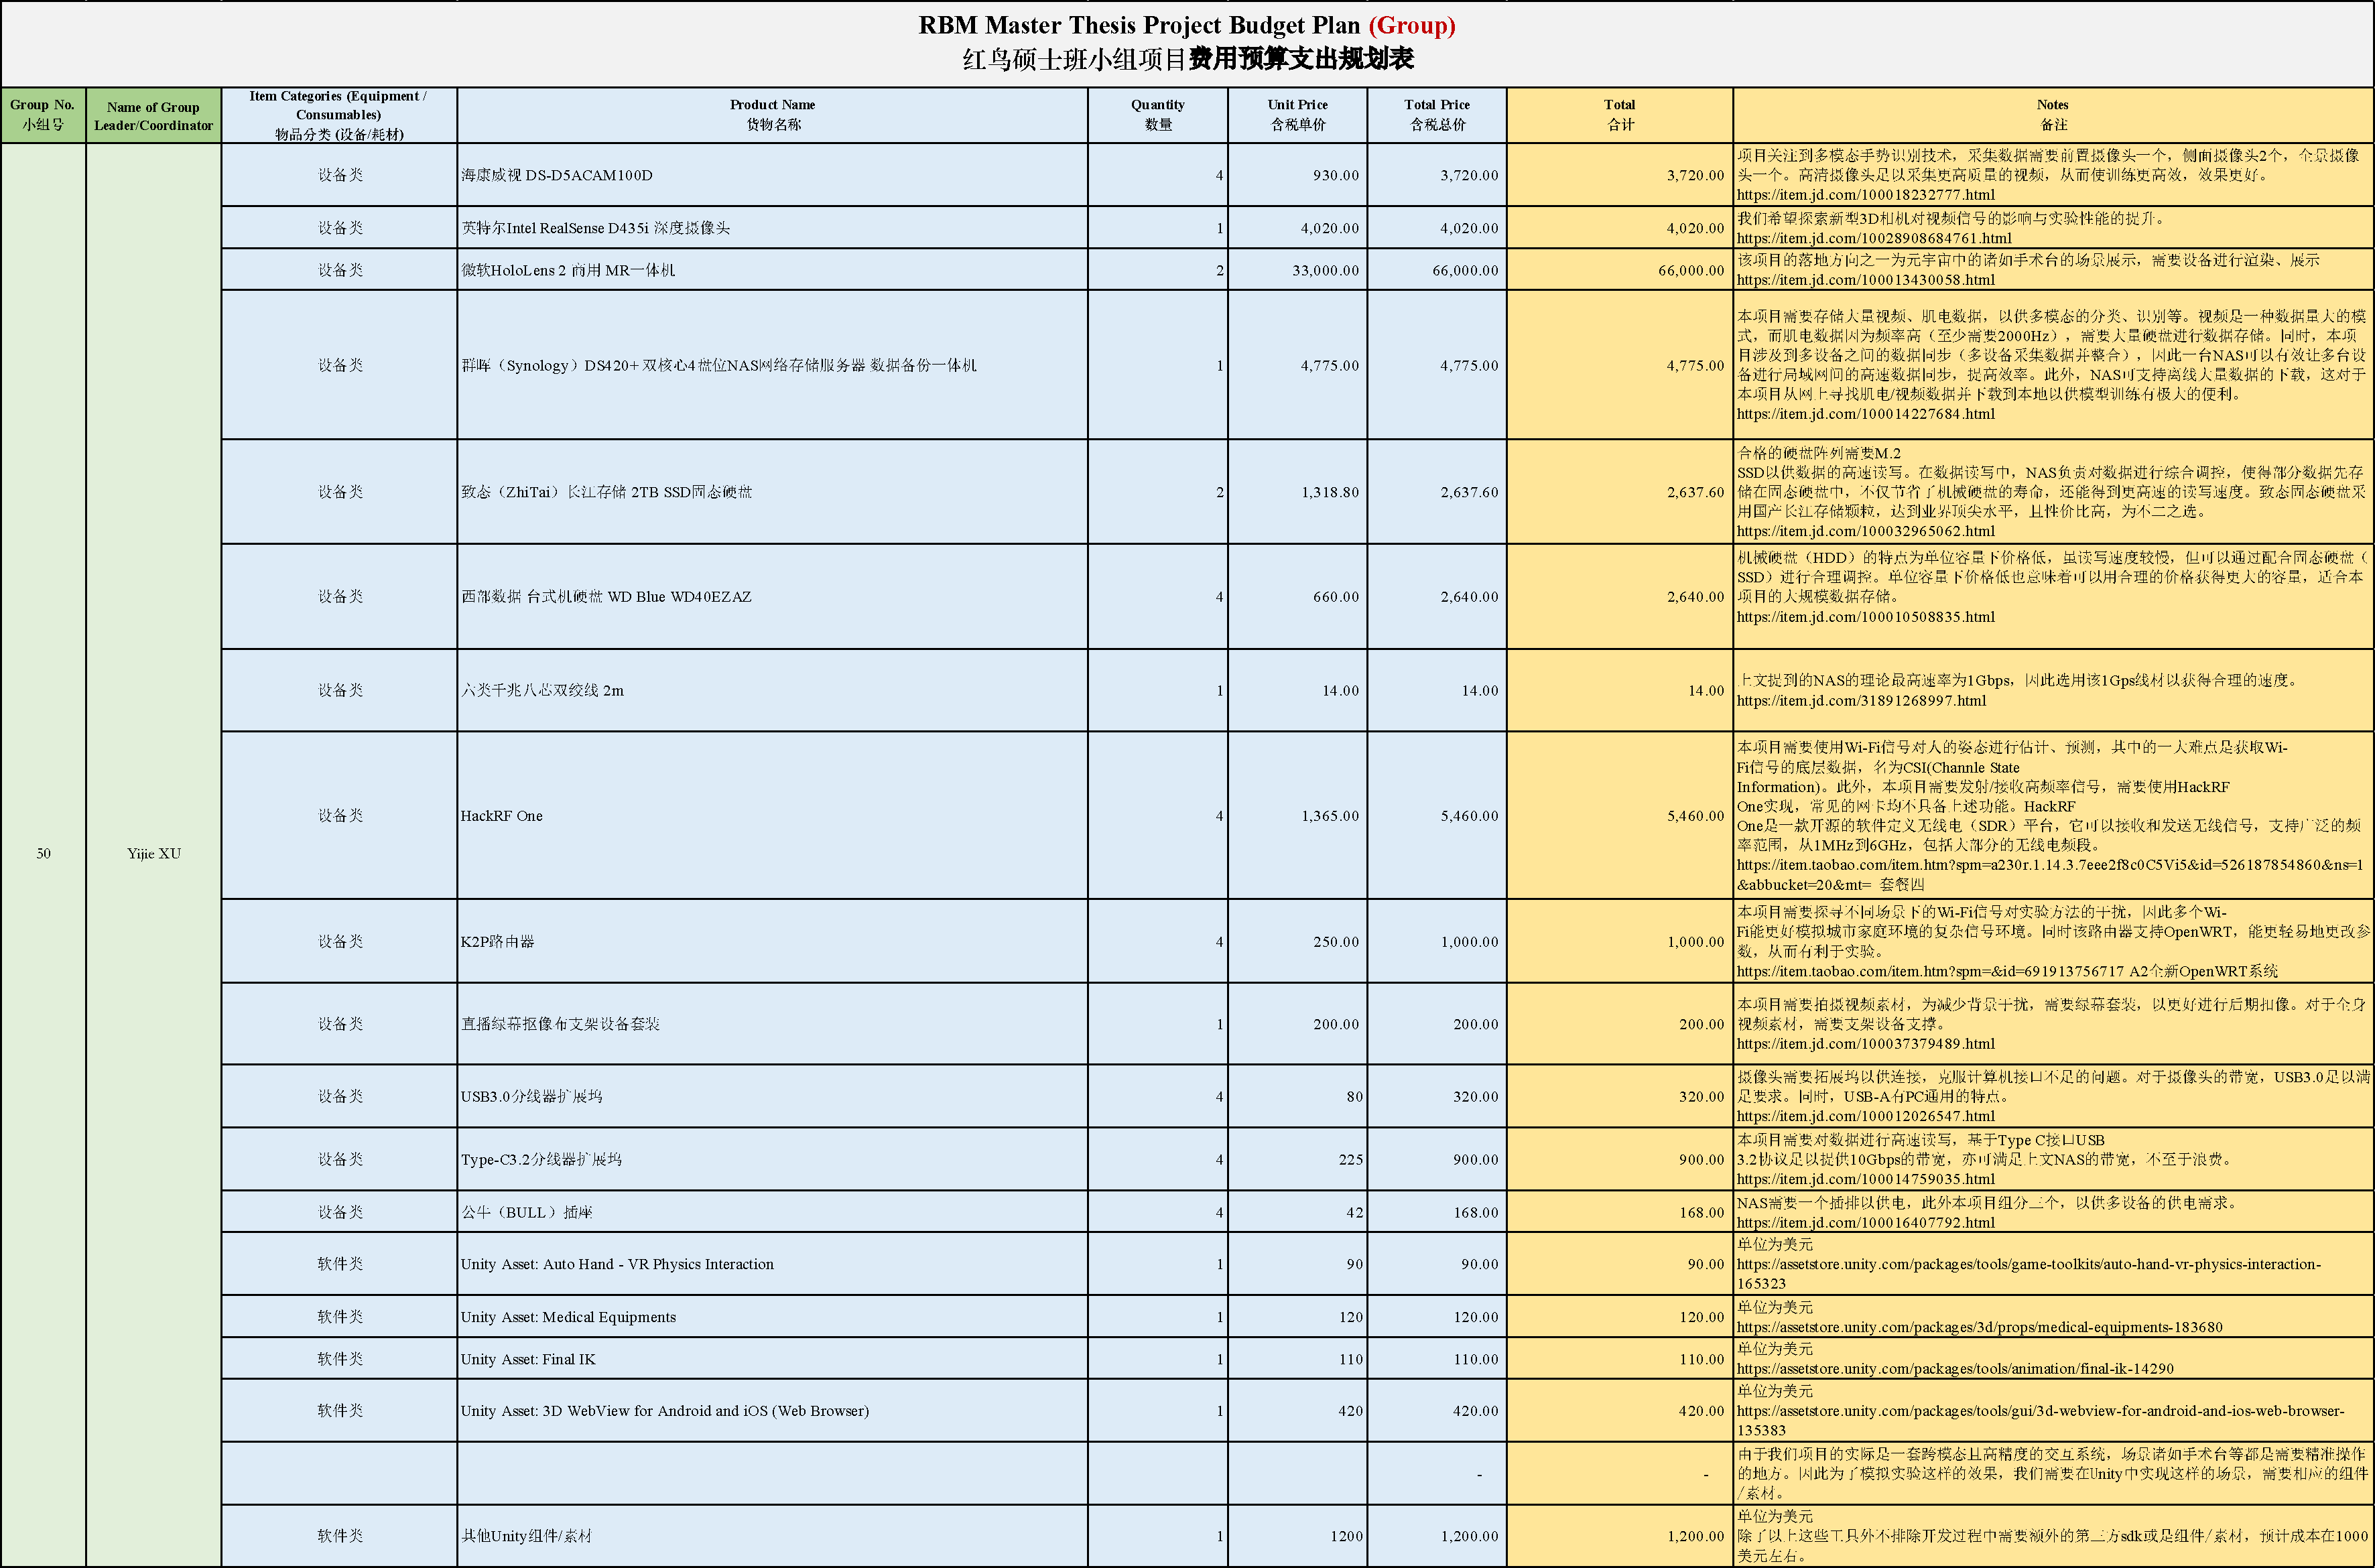
\includegraphics[width=0.6\textwidth]{image/budget_plan.pdf}
    \caption{Part of the budget plan to RBM}
    \label{fig:budget_plan}
\end{figure}


\begin{figure}[ht!]
    \centering
    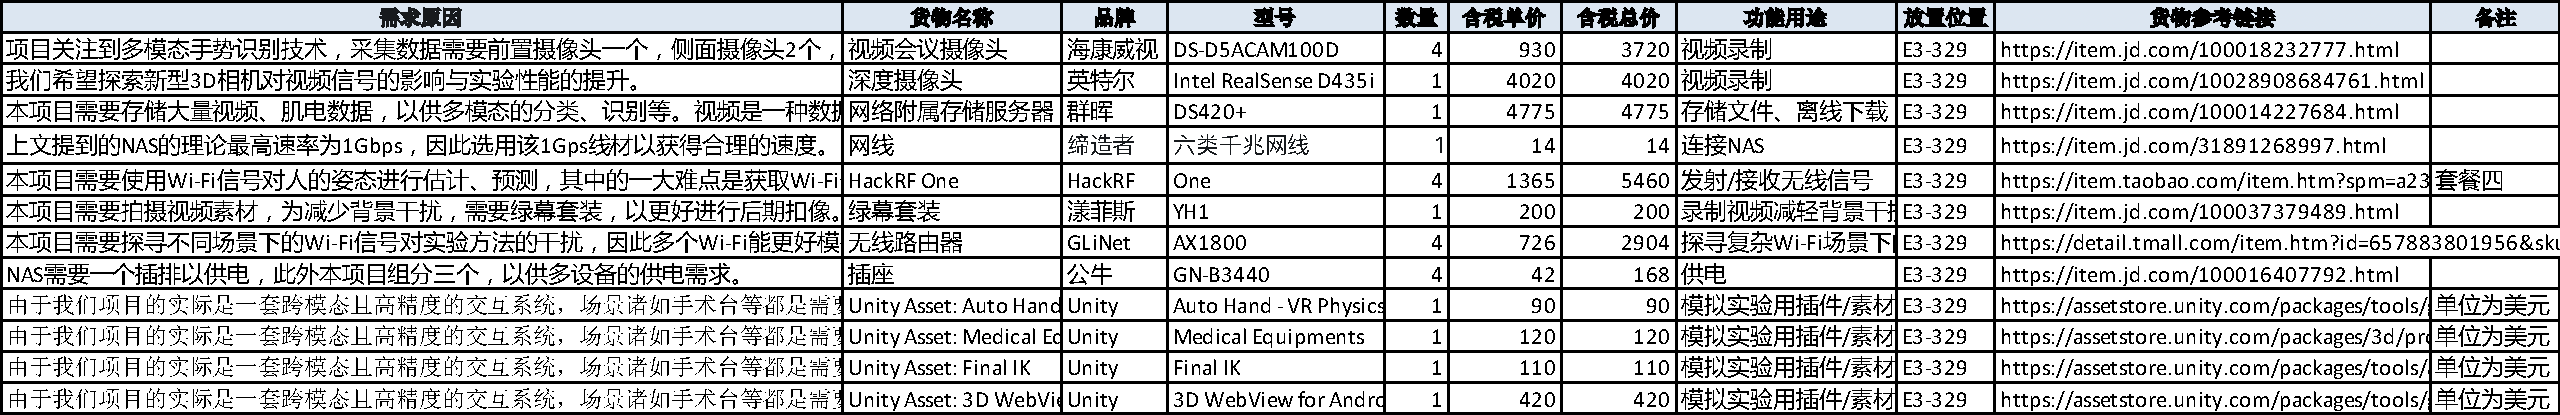
\includegraphics[width=1.0\textwidth]{image/procurement.pdf}
    \caption{Part of the procurement application to RBM}
    \label{fig:procurement}
\end{figure}

Moreover, the effective implementation of our experimental design necessitates the availability of spacious environments. Specifically, each of the three modalities of sensors we plan to utilize requires adequate space to operate optimally. For instance, the transmission of Wi-Fi signals requires a designated room. Similarly, the operation of individuals with surface electromyography (sEMG) sensors entails ample room to perform different actions. Additionally, the procurement of a green screen necessitates a sizable area for its placement and the installation of accompanying cameras.

\newpage
\section{Anticipated Problems and Solutions}
In the course of undertaking this research project, we anticipate encountering several challenges that may impede our progress. However, we have proactively devised strategies to mitigate these issues and facilitate a smooth research process.

\begin{enumerate}
\item Hardware-Software Compatibility Issues with Wi-Fi Signals: We anticipate potential compatibility issues between the hardware (HackRF One\cite{ossmann2018hackrf}) and software (PicoScenes\cite{jiang2022picoscenes}) components of our Wi-Fi signal processing system. These challenges may arise due to limited documentation and tutorials available for integrating these components. To address this, we plan to engage the software author on GitLab by submitting detailed issues outlining our concerns. Moreover, we will explore relevant literature, technical forums, and online communities to gather insights and potential solutions from experts in the field.

\item Uneven Task Distribution within the Research Group: A heterogeneous distribution of tasks among the group members may lead to inconsistencies in the completion status of individual assignments. To mitigate this, we will establish a structured communication framework that includes regular group meetings, progress updates, and collaborative task management. This will enable us to synchronize our efforts, maintain transparency, and ensure that all group members are actively contributing to the project's objectives.

\item Procurement Process Delays: The procurement of essential equipment and components may be hindered by lengthy institutional procedures and administrative protocols, potentially delaying the establishment of our experimental platform. To circumvent this issue, we will engage in proactive communication with the relevant administrative personnel to expedite approval processes. Additionally, we will explore alternative sourcing strategies, such as reaching out to industry partners or leveraging existing resources within the institution, to ensure timely acquisition of the required items.
\end{enumerate}

We possess a firm conviction that the obstacles we currently face can be surmounted. Our research project is aimed at achieving a dual purpose of academic excellence and practical engineering applications. We are confident that through our diligent efforts and systematic approach, we can attain this goal.

We recognize the challenges that may arise during the course of our research project, but we are committed to overcoming them with the utmost determination and perseverance. Our project embodies a rigorous and comprehensive investigation of the subject matter, which will be meticulously documented and evaluated to ensure its scholarly value.

Moreover, we are driven to make a significant impact beyond the academic realm by contributing to the engineering community with practical and applicable solutions. We are confident that our findings will be highly regarded and embraced by professionals in the field.

In summary, we are dedicated to executing our research project with excellence, rigor, and innovation. We firmly believe that our work will bridge the gap between academic excellence and practical engineering applications and will be highly regarded by both the academic and engineering communities.


\newpage
% \bibliography{jpp-instructions}
\printbibliography
% \bibliography{reference/reference2}


\end{document}
